%\newpage

\section{Results and Discussion}
The analysis and calculations were conducted using the R programming language \cite{R} version 4.3.2 and Python Jupyter Notebooks \cite{IPython:2007} running Python version 3.7.9 and the latest package versions available on January 12, 2024. The scripts are included in the appendix of this report. \ref{r_scripts} All uncertainties stated are provided for a 95 \% confidence interval, in accordance with the ISO guide to the uncertainty of measurements (GUM)\cite{GUM} and this courses guidelines\cite{meister}.


\subsection{Density and refractive index}

The refractive index and density of acetone were measured at 

$n_D^{20} =$ \qty{1.35867}{1} and 

$\rho = $ \qty{0.7913}{\density} (\textit{method B}) 
\\and the density of acetone was calculated (\textit{method A}) to be 

\qty{0.790 \pm 0.003}{\density} 
\\corresponding with literature values of 

$n_D^{20} =$ \qty{1.3588}{1} and 

$\rho = $ \qty{0.7899}{\density}. \cite{meister} 
\\For n-hexane values of 

$n_D^{20} =$ \qty{1.37506}{1} and 

$\rho = $ \qty{0.6594}{\density} (\textit{method B}) and 

$\rho = $ \qty{0.6572 \pm 0.0022}{\density} (\textit{method A}) 
\\were obtained compared to literature values of 

$n_D^{20} =$ \qty{1.3751}{1} and 

$\rho = $ \qty{0.6603}{\density}. \cite{meister} 
\\It can be observed, that the results obtained for acetone are more precise than those of n-hexane. This could be explained for example by the varying grades of purity (99.5\% vs. 95\% specified by their producers.
\begin{figure}[H]
    \centering
    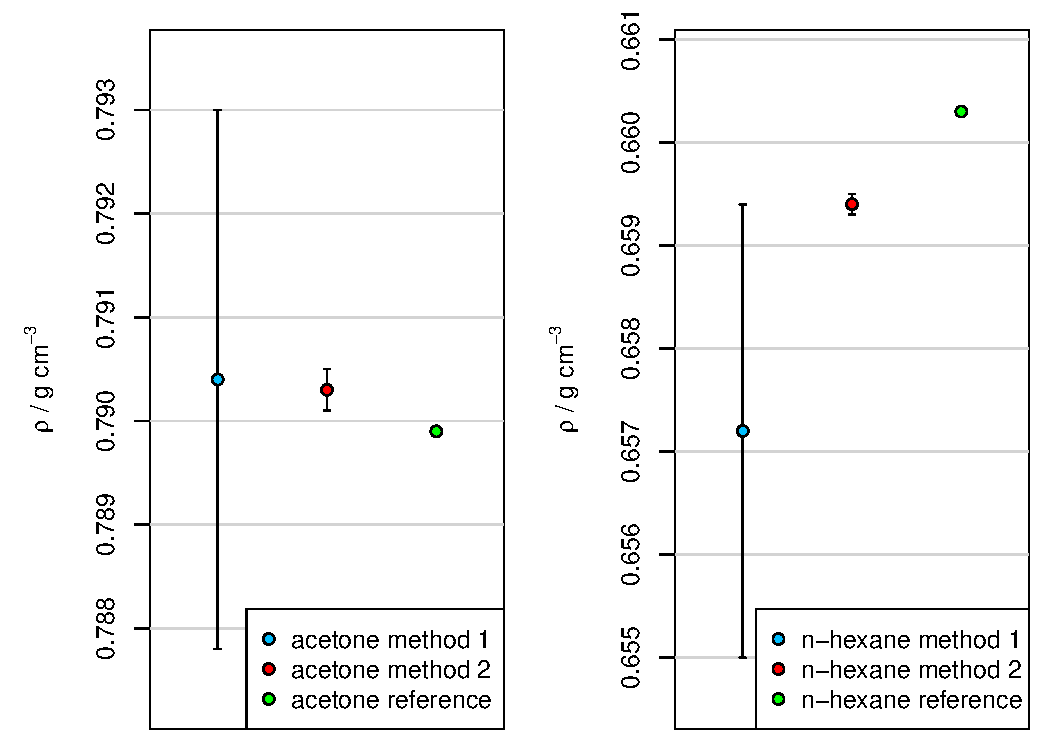
\includegraphics[width=.5\textwidth]{figures/rho-comparison.pdf}
    \caption{Comparisons of the density values measured, and reference values found in literature \cite{meister}.}
    \label{fig:rho_comp}
\end{figure}


\subsection{Vapor Pressure}

\begin{figure}[H]
    \centering
    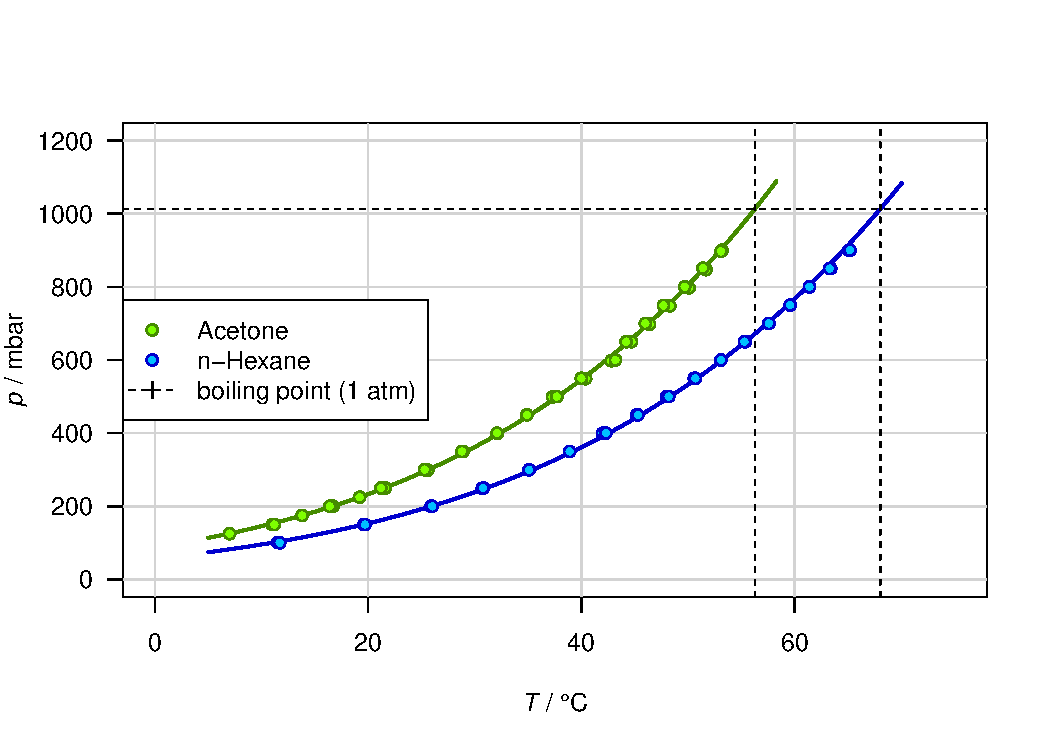
\includegraphics[width=.5\textwidth]{figures/DDR1_t_p.pdf}
    \caption{The vapor pressure curves illustrate the exponential correlation between vapor pressure and temperature. (Standard boiling points extrapolated and marked by the vertical and horizontal lines.)}
    \label{fig:ddr1_t_p}
\end{figure}

As mentioned in the introduction, vapor pressure can be described as $p(T)$. Accordingly, the results obtained from measuring the samples' boiling temperatures at differing surrounding pressures were plotted in a $p$-$T$-diagram, presented in Fig. \ref{fig:ddr1_t_p}.

Enthalpies of vaporization were calculated with by plotting logarithmic $\frac{p}{p_0}$ against inverse temperature $T$ via a linear regression model (Fig. \ref{fig:ddr1_inv_ln}) and calculating the slope $b$ of the resulting linear graphs. Expansion of equation (\ref{eq:6.2}) shows that it is equal to $\frac{\Delta_VH}{R}$. Results amounted to 

$\Delta_VH=$ \qty{32.5 \pm 0.3}{\kJpmole} for acetone and 

$\Delta_VH=$ \qty{32.7 \pm 0.3}{\kJpmole} for n-hexane. 
\\Acetone is a polar solvent and n-hexane is not. Because of this, one would assume, that its enthalpy of vaporization and standard boiling temperature would be higher than those of n-hexane because of stronger intermolecular bonds. Evidently, this is not the case. A possible explanation could be that though it is polar, acetone has a lower molar mass than n-hexane, meaning it would take less  energy to bring one mol of acetone from its fluid to its gaseous form than one mol of another substance with similar polarity.

 
\begin{figure}[H]
    \centering
    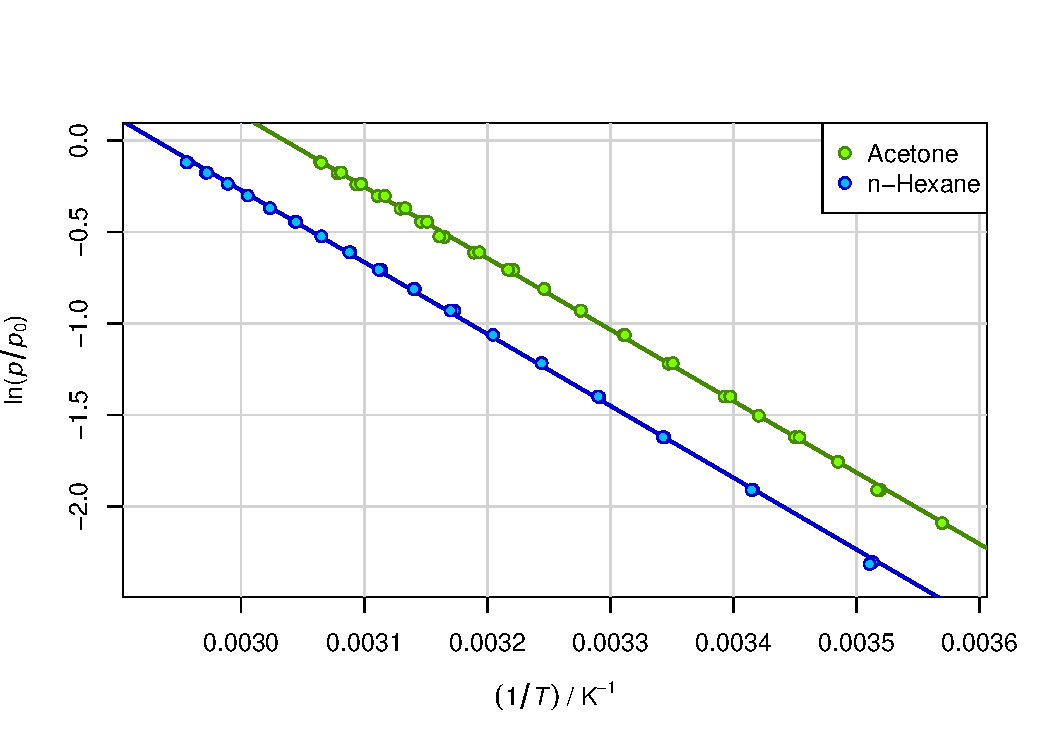
\includegraphics[width=.5\textwidth]{figures/DDR1_inv_ln.pdf}
    \caption{The Enthalpy of vaporization for each sample can be visualized in a $\ln\left(\frac{p}{p_0}\right)$ - $\frac{1}{T}$ diagram, because it is directly proportionate to the linear graph's slope $b$ (by factor of the gas constant $R$.)}
    \label{fig:ddr1_inv_ln}
\end{figure}


Normal boiling temperatures $T_0$ and standard entropies $\Delta_VS(T_0)$ of vaporization were also calculated with the help of the linear model parameters intercept $a$ and slope $b$ and found to be 

$T_0^{\text{acet}}$ = \qty{56.29}{\celsius}  

$T_0^{\text{nhex}}$ = \qty{68.06}{\celsius}
\\corresponding to literature values of 

$T_0^{\text{acet}}$ = \qty{56.2 \pm 0.3}{\celsius} 

$T_0^{\text{nhex}}$ = \qty{68.8 \pm 0.3}{\celsius}
\\and

$\Delta_VS(T_0)^{\text{acet}}$ = \qty{98.6 \pm 0.8}{\joule\per\mole\per\kelvin}

$\Delta_VS(T_0)^{\text{nhex}}$ = \qty{95.7 \pm 0.8}{\joule\per\mole\per\kelvin}.





\subsection{Transient evaporation cooling}
The data files generated by the \texttt{TREVAC} apparatus were imported to R. With the \mintinline{R}{identify()} command, the relevant time ranges for the peak integration could be selected graphically. (Fig. \ref{fig:nhex_peaks}) This data, including statistical parameters were then exported to a \textit{csv} file for documentation purposes and for further processing. To calculate the final values, including standard errors, a Jupyter notebook \cite{IPython:2007} with the \texttt{METAS UncLib} uncertainty modeling software \cite{unclib} was used.

For acetone, \qty{30.2 \pm 2.8}{\kJpmole} was calculated, and for n-hexane, \qty{32.0 \pm 1.9}{\kJpmole}, was found.

\begin{figure}[H]
    \centering
    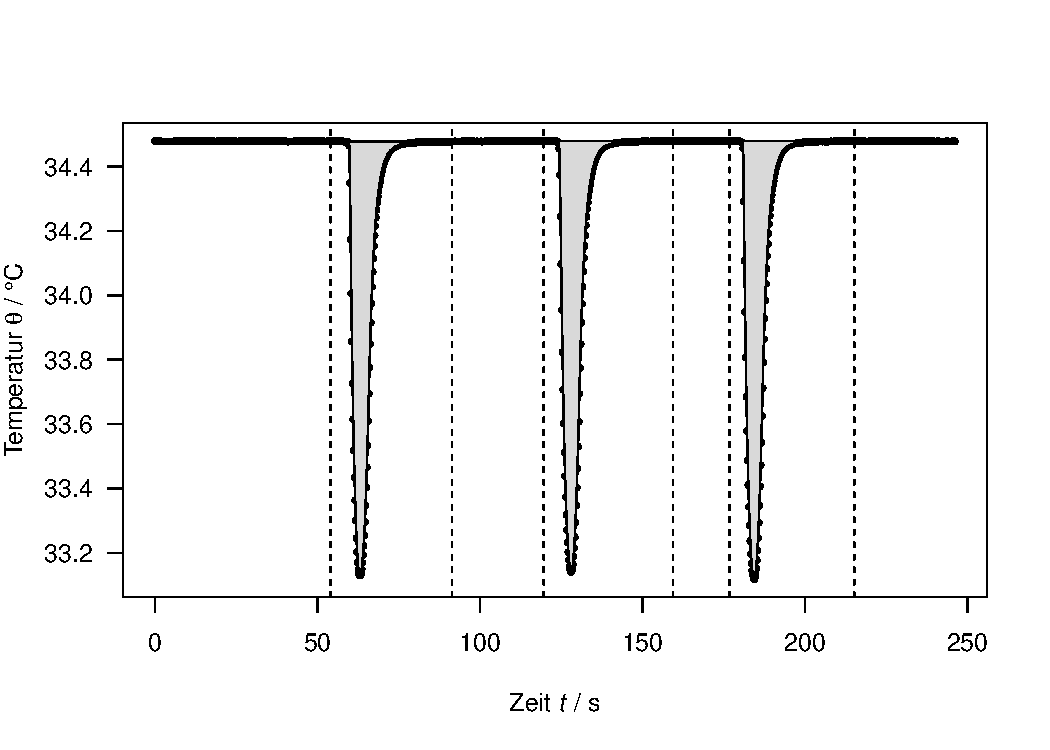
\includegraphics[width=.5\textwidth]{figures/n-hexane.pdf}
    \caption{Temperature peaks caused by n-hexane withdrawing heat from the measurement surface. The grey area is directly correlating with the enthalpy of evaporation $\Delta_VH_{\text{subst}}$ of the substance.}
    \label{fig:nhex_peaks}
\end{figure}

Standard values for $\Delta_VH$ can be found on the website of the \texttt{National Institute of Standard Technology}:

$\Delta_VH^0_{\text{acet}}$ = \qty{31.27}{\kJpmole} \cite{NIST:acet}

$\Delta_VH^0_{\text{nhex}}$ = \qty{31\pm 1}{\kJpmole} \cite{NIST:nhex}

